\label{chapter-4}

\noindent In this chapter, I introduce {\tt eth2dgraph}, the new open-source software designed to facilitate the extraction and indexing of Ethereum data in Dgraph.

Eth2dgraph is developed using Rust, a system programming language that prioritizes both speed and safety. Rust was chosen mainly for two reasons. Firstly, for its emphasis on performance and parallelism, crucial for scaling the data extraction process and achieving good performance. Secondly, Rust benefits from a rich ecosystem of libraries specifically designed for handling Ethereum data, easing the process of development.

One of the key features of eth2dgraph is its integration with a decompiler, enabling the extraction at the scale of the Application Binary Interface (ABI) from the bytecode stored on the Ethereum blockchain. 

The following sections provide details about the architecture of eth2dgraph, give a comprehensive overview of how the software operates, and how it has been constructed.

\section{Data flow}

Extracting and indexing Ethereum Smart Contract data is a process of moving and transforming bytes. Raw data stored in the Ethereum node must be taken, transformed and ingested into a database, Dgraph in this case, in order to be indexed. 

The first attempt was to do this step through transactions. I ran a Dgraph cluster and instructed eth2dgraph to add data via DQL mutations. DQL stands for \textbf{Dgraph Query Language} and it is the language used to write Dgraph queries. This data flow was working but it was too slow for thinking about applying it to all the history of the Ethereum chain. I also had problems to parallelize data insertion, too many concurrent transactions were failing due to read-write conflicts. \cref{fig:data-flow-1} visualizes this data flow.

\begin{figure}[H]
\centering
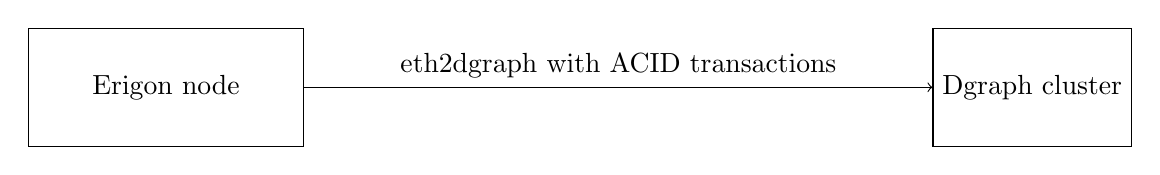
\begin{tikzpicture}
    \node[draw,minimum width=35mm,minimum height=15mm] (erigon) at (0,0) {Erigon node};
    \node[draw, minimum width=25mm,minimum height=15mm] (dgraph) at (11,0) {Dgraph cluster};
    \draw[->] (erigon) edge node[sloped, above] {eth2dgraph with ACID transactions} (dgraph);
\end{tikzpicture}
\caption[First attempt of data ingestion into Dgraph]{First attempt of data ingestion into Dgraph}
\label{fig:data-flow-1}
\end{figure}

To solve these problems, I changed the approach and followed an ETL (Extract, Transform, Load) process. Extraction and transformation are done in the same step by eth2dgraph. The output is stored in JSON files that can be later loaded into Dgraph using the Bulk Loader.

The Bulk Loader\footnote{Detailed description of the Bulk Loader: \url{https://dgraph.io/blog/post/bulkloader/}} is a tool provided by Dgraph. It is designed for performing the initial load of data into the database. It takes JSON or RDF N-Quads\footnote{N-Quads is a serialization format for RDF graphs data \url{https://www.w3.org/TR/n-quads/}.} data and stores it directly in Badger, the underlying key-value database used by Dgraph. This is the fastest way to ingest data into Dgraph. It maximizes concurrency and avoids problems related to ACID constraints since it is not operating on a live database. \Cref{fig:data-flow-2} visualizes the final data flow chosen for eth2dgraph.

\begin{figure}[H]
\centering
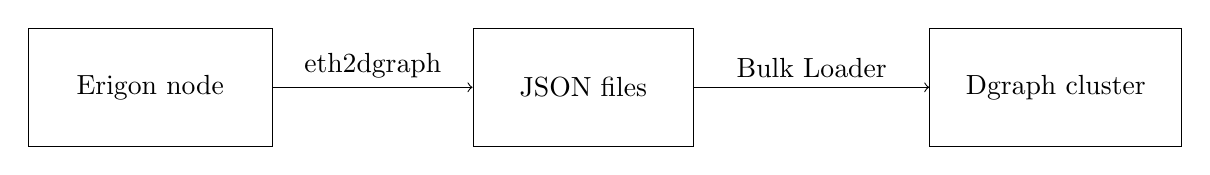
\begin{tikzpicture}
    \node[draw,minimum width=31mm,minimum height=15mm] (erigon) at (0,0) {Erigon node};
    \node[draw, minimum width=28mm,minimum height=15mm] (json) at (5.5,0) {JSON files};
    \node[draw, minimum width=32mm,minimum height=15mm] (dgraph) at (11.5,0) {Dgraph cluster};
    \draw[->] (erigon) edge node[sloped, above] {eth2dgraph} (json);
    \draw[->] (json) edge node[sloped, above] {Bulk Loader} (dgraph);
\end{tikzpicture}
\caption[Second and final data flow]{Second and final data flow}
  \label{fig:data-flow-2}
\end{figure}

\section{Data model}

After seeing how data is indexed in other works, I decided to design the schema in a slightly different way. In eth2dgraph, raw data is interpreted to create a schema around the semantics that can be extracted from the blockchain. This semantics is indexed alongside the raw Ethereum data. \Cref{fig:schema} shows the whole schema that was created. All the edges have the {\tt @reverse} index, which means they can be traversed in both directions. Some of the attributes are indexed at load time, but it is easy to add indexes once the database is running. The complete description of both DQL and GraphQL schemas are described in~\cref{app-b}.

% TODO: update schema with final version

\begin{figure}[H]
  \centering
  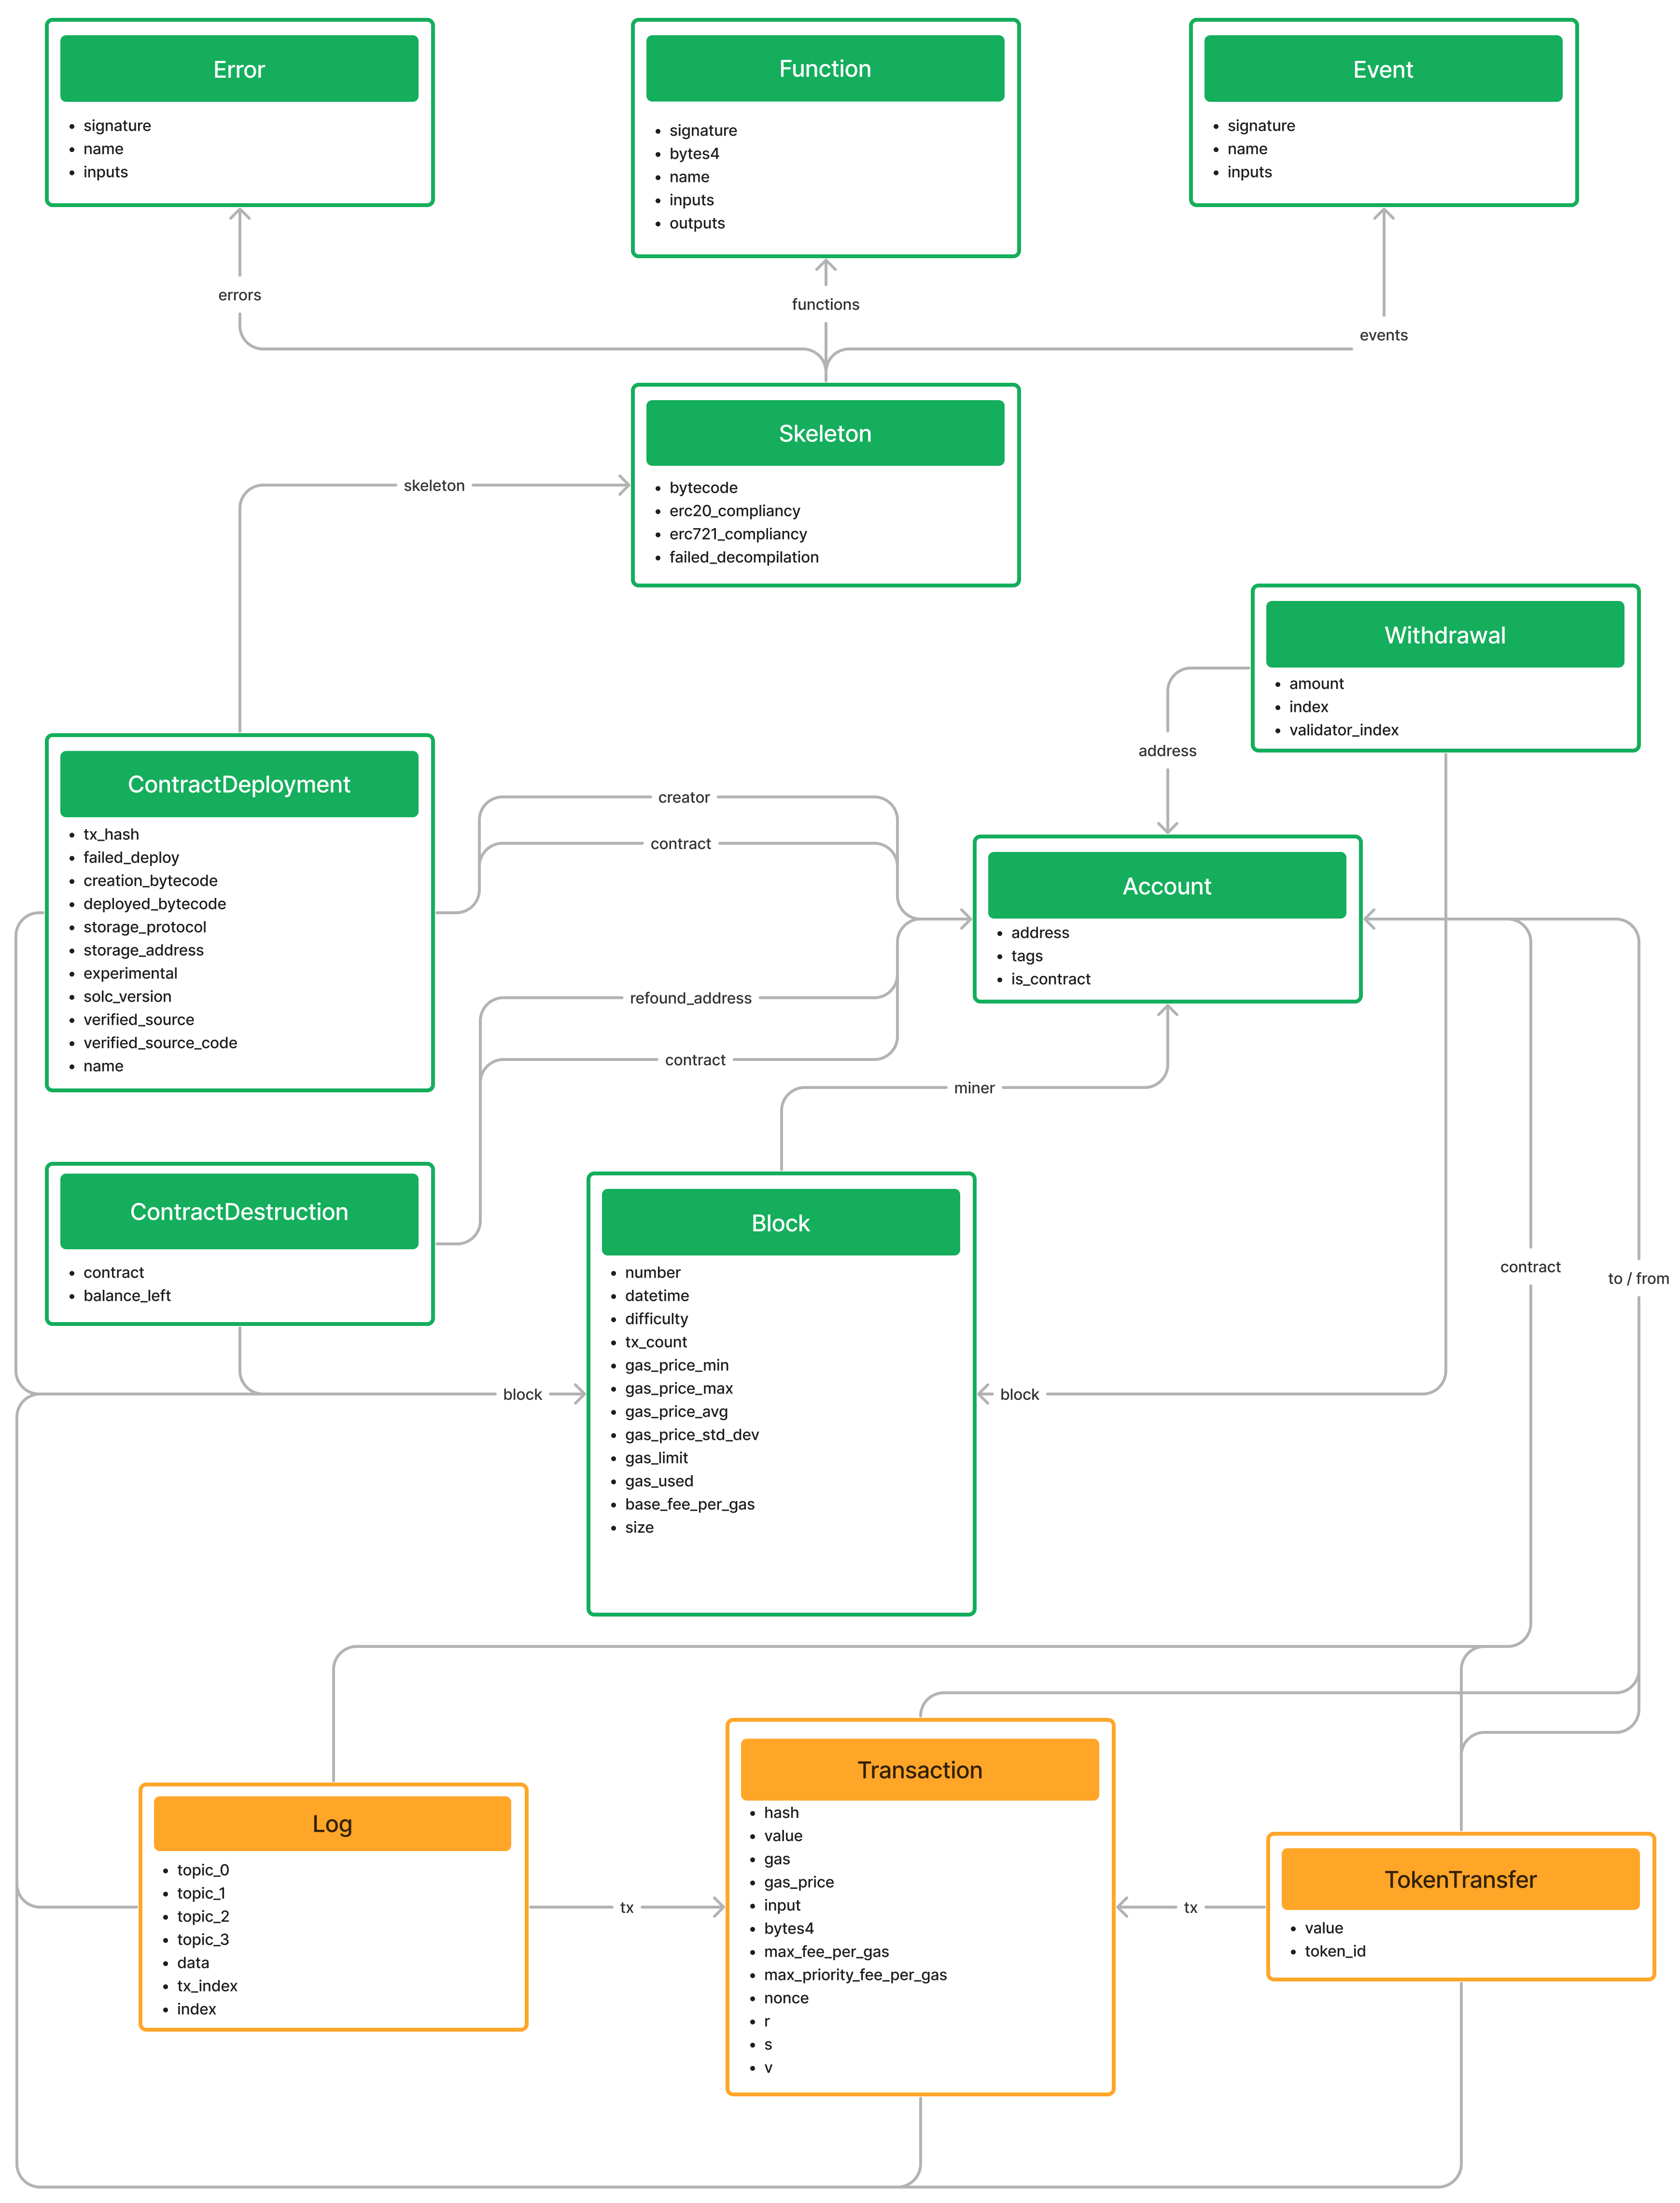
\includegraphics[width=1\textwidth]{Figures/methods/schema.png}
  \caption[Schema of Ethereum indexed data in Dgraph]{Schema of Ethereum indexed data in Dgraph}
  \label{fig:schema}
\end{figure}

Data is modelled as a graph with many edges. This was done since Dgraph is designed and optimized to perform joins and traversals.

Entities in yellow (\textit{Transaction}, \textit{TokenTransfer} and \textit{Log}), also called \textit{dynamic}, are optional and can be skipped during data extraction. Excluding data about smart contracts usage allows the creation of a much smaller dataset that provides a static description of these contracts. The reason of this choice is that the volume of dynamic data is around {\tt 30-40x} bigger than static data. Having the option to extract a smaller dataset enables analysis on less powerful computers, improving the accessibility of the research. \\

\noindent Here is a brief description of the schema:

\begin{itemize}

    \item \textit{Transaction} and \textit{Log} are stored as they are retrieved from the Ethereum node. References to other entities are stored as edges for allowing graph traversal in queries. A \textit{Transaction} represents a transfer of value between two EOAs or an invocation of a Smart Contract from an EOA. A \textit{Log} is the result of an invocation of an Event in the code of a Smart Contract.

    \item \textit{TokenTransfer} represents both an ERC20 or an ERC721 token transfer between two accounts. The value is stored as a string since Dgraph does not handle 256-bit integers.
    
    \item \textit{Block} contains all the information related to a single Ethereum block header. This entity is connected to many others: \textit{ContractDeployment}, \textit{ContractDestruction}, \textit{Transaction}, \textit{TokenTransfer} and \textit{Log}. 
    
    The indexed attribute \textit{datetime} is the only reference to time in the database, so it is possible to query it for specific dates and times and then get all the connected data from there. 

    Here, it added a summary of the gas prices of the transactions included.

    \item \textit{Withdrawal} represents a withdrawal from a validator. Withdrawals are used to remove the locked funds and stop being a validator in the proof of stake.

    \item \textit{Account} represents an Externally Owned Account or a Contract Account. Its fundamental attribute is the \textit{Address} of the account. There is also a boolean field \textit{is\_contract} indicating whether the account is a contract or not. This entity is extremely useful for querying data since with the standard Ethereum RPC interface it is not possible to query data based on account addresses. So, for example, it is impossible to get all the transactions from/to an address without having to download and filter all the transactions in the history of Ethereum.

    \item \textit{ContractDeployment} and \textit{ContractDestruction} represent respectively the birth and the death of the code of a Smart Contract. I decided to store them in this way since I found, analyzing the data, that a single Ethereum Address can receive more than one code deployment, contrary to what it may appear because of the theoretical immutability of Smart Contracts. An address can receive both a deployment with the same old code or with a new different code, in which case it is called \textit{morphic} or \textit{metamorphic}~\cite{create2-metamorphic}.

    \item I introduced the concept of \textit{Skeleton} directly in the schema since it is a useful way of aggregating similar contracts together. A \textit{Skeleton} is the bytecode of a contract without all the arguments of the PUSH opcodes. Having it directly in the schema allows us to easily find contracts sharing the same skeleton.

    \item \textit{Event}, \textit{Function} and \textit{Error} are the parts that, together, form the ABI of the contracts. There is just one entity for each signature, so all the contracts implementing the same function/event/error point to the same entity. Having them indexed in this way allows to search contracts based on the functionalities they implement.
    
\end{itemize}

\section{Data extraction}

Data is extracted using the Ethereum \textit{Remote Procedure Call} (RPC) interface\footnote{Official specification of the Ethereum RPC interface: \url{https://ethereum.github.io/execution-apis/api-documentation/}}. Eth2dgraph extracts data block by block. It needs three API calls per block to get all the data: \texttt{eth\_getBlockByNumber}, \texttt{eth\_getLogs} and \texttt{trace\_block}. 

To call these RPCs, I used the Rust library \texttt{ethers-rs}\footnote{\url{https://docs.rs/ethers/latest/ethers/}}, which provides, among other functionalities, a full client implementation that wraps the standard Ethereum RPC interface and provides easy methods to interact with it in an asynchronous runtime.

At a high level, data returned from these RPC endpoints is parsed into Rust structs and later serialized into JSON files using the \textit{serde}\footnote{Serde is a Rust framework for easily serializing and de-serializing data structures \url{https://github.com/serde-rs/serde}} crate. To implement this, all the Rust structs that must be serialized to Dgraph format implement a trait called \textit{SerializeDgraph}. In Rust, a trait defines a collection of methods. A struct that implements a trait is guaranteed to have those methods implemented. It is a concept similar to the Interfaces in object-oriented programming (OOP) languages.

The trait \textit{SerializeDgraph} requires one method to be implemented:\\ \texttt{serialize\_dgraph}. As the name suggests, it is a function that serializes a generic struct to the JSON format accepted by the Dgraph Bulk Loader.

The entities produced by eth2dgraph are linked together using the Dgraph's \textit{blank nodes}. It is a way of referencing to an entity that has yet to be created. Dgraph will resolve all the references to a blank node generating and using the same \texttt{uid}.

The next sections explain how each piece of data is extracted.

\subsection{Blocks and transactions}

Blocks and transactions are both extracted from the data returned by the RPC \texttt{eth\_getBlockByNumber}. 
This method accepts two parameters:

\begin{itemize}
    \item \textit{Block number} specifies the target block that is extracted
    \item \textit{Hydrated transactions} is a boolean indicating whether to return or not all the details of the transactions in that block.
\end{itemize}

Eth2dgraph calls this RPC sequentially for each block with \textit{Hydrated transactions} set to \texttt{true}. All raw transaction data is stored without modifications, same for the withdrawals. For the blocks I added a summary of the gas price, this is not returned by  default from the RPC. These fields have been added: 

\begin{itemize}
    \item \textit{gas\_price\_min}: the cheapest gas price of all the transactions included in the block, in Gwei.
    \item \textit{gas\_price\_max}: the maximum amount paid for gas in the transactions included in the block, in Gwei.
    \item \textit{gas\_price\_avg}: the average price of gas in Gwei of that block.
    \item \textit{gas\_price\_std\_dev}: the standard deviation of gas price in that block, in Gwei.
\end{itemize}

Gas price varies between each transaction. Sticking to the official RPC docs, it should be possible to obtain data about it just from the transaction receipts. This would imply getting more data and slowing down the process of data extraction.

Looking at the data returned from the Erigon node and analyzing its source code\footnote{\url{https://github.com/ledgerwatch/erigon/blob/35422986645832d1c9ce1107a59dbaf4e12f55dd/turbo/adapter/ethapi/api.go\#L450}}, I noticed that gas price was present even if not required by the protocol. I compared it to the data returned from the receipts and it matched, so I decided to use it and store this information in the database.

\subsection{Logs}

Logs are retrieved using the \texttt{eth\_getLogs} RPC. This remote procedure call accepts an object as a parameter, it can be used as a filter to refine the call and get just the logs needed. It is possible to filter by topics, contract address and block range. 

All the logs are already indexed in the Ethereum nodes by the fields on which it is possible to filter. It is the standard way to extract semantics from the chain. When specific conditions happen inside a call to a smart contract, it can emit a log with up to four indexed 256-bit words that will be stored by all the Ethereum nodes. These logs can represent any kind of information, e.g.~token transfers, and token swaps.

Eth2dgraph is getting logs and downloading them block by block. The RPC \textit{eth\_getLog} is called for each block with a filter on the blocks range, with matching \textit{fromBlock} and \textit{toBlock} parameters.

\subsection{Smart contracts}

There are two ways to deploy a smart contract on the Ethereum blockchain: 

\begin{itemize}
    \item From EOAs, with a transaction to the address \texttt{0x0} containing as input data the deployment code of the smart contract.
    \item From other smart contracts, calling the EVM opcode \texttt{CREATE} or \texttt{CREATE2}, after having pushed on the stack the deployment code of the smart contract to deploy.
\end{itemize}

There is no RPC to directly get the list of contracts. Smart contracts are not indexed by the Ethereum nodes.

It is relatively easy to extract smart contracts deployed in the first way, it is enough to loop through transactions and see the ones sent to the address \texttt{0x0}. The resulting transactions are potential contract deployments. To confirm this, it is possible to download their receipts, which contain the address of the newly created contract in case the deployment is successful. After finding the address, it is possible to get the deployed bytecode calling the RPC \texttt{eth\_getCode}, which returns the actual code stored on the blockchain.

This way of extracting contracts has two drawbacks: it requires two extra calls to RPCs for each deployment and it misses all the contracts deployed by other contracts. Contracts are more likely to be deployed by other contracts rather than by users~\cite{ethereum-sc-topology}, so it is clear that this way is not ideal.

To extract all the contract deployments, it is necessary to inspect each individual interaction done on the blockchain, both between users and contracts (via transactions) and between contracts and other contracts (via \textit{internal transactions}). 

Internal transactions (also known as \textit{traces}) are the result of a call to a smart contract, they describe each single operation performed in that call. They are not described in the Ethereum Yellow Paper~\cite{ethereum-yellow} and they do not need to be stored by the nodes. They are just a detailed description of a transaction execution. They can be calculated having the transaction data, the bytecode to be executed and the state of the blockchain at the time of the transaction execution. 

Erigon provides a RPC to collect all the traces of all the transactions in a block, it is called \texttt{trace\_block}. Traces returned can be of four types: \textit{Call}, \textit{Create}, \textit{Suicide} and \textit{Reward}. They are structured as a directed graph: an internal transaction can generate many other internal transactions. To get deployments and destructions, it is sufficient to go through the traces graph and filter the Create and Suicide traces, they contain all the needed information.

Eth2dgraph is using the \texttt{trace\_block} RPC to collect all the deployments and destructions of smart contracts.

\subsection{Error propagation in traces}

An Ethereum transaction can be successfully executed even if some of its parts have failed. An error in one internal transaction implies that all its child traces have no effect on the blockchain. 

\begin{figure}[!ht]
  \centering
  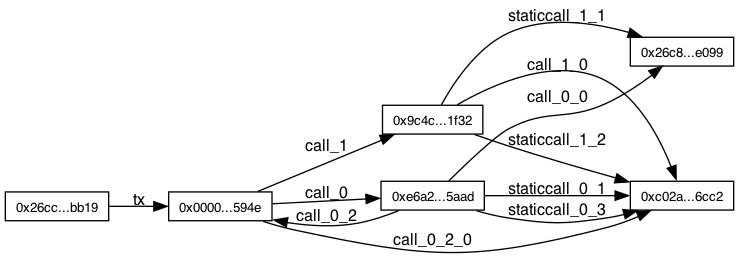
\includegraphics[width=1\textwidth]{Figures/methods/traces.png}
  \caption{Example of the structure of traces in a transaction.}
  \label{fig:traces}
\end{figure}

\cref{fig:traces} gives an example of the structure of traces in the transaction {\tt 0x7b4968c606e...4d941d66977}\footnote{Full tx hash: 0x7b4968c606e100d05158456d66d620ff6e96f00d68e3b6a426b774d941d66977}. Supposing that {\tt call\_1} failed, all its child calls ({\tt call\_1\_0}, {\tt staticcall\_1\_1} and {\tt staticcall\_1\_2}) will not change the state of the blockchain, despite being included in the traces returned by {\tt trace\_block}. Contracts deployed or destructed in an internal transaction that is part of a failed branch will not be effectively deployed or destroyed. 

The only reference to the error is present in the single trace that failed, with an {\tt error} field. To understand if a deployment or a destruction successfully completed, it is necessary to propagate the error from the failed traces to all its children. Eth2dgraph does so with the algorithm reported in \cref{lst:error-propagation}. It first groups traces of a block based on transaction hash. Then, for each transaction, it gets its failed traces. Then it loops again on all the traces of the transaction to see if any of them is a child of a failed one. This is done by searching a failed trace that has a matching starting address, e.g. a trace with address {\tt 1, 0, 0} has a matching starting address of the trace {\tt 1, 0, 0, 2}.

Contract deployments and destructions found in failed traces are stored in the output of eth2dgraph with a boolean field indicating it.

\begin{lstlisting}[language=Rust,caption={Algorithm for errors propagation in traces.},label={lst:error-propagation},captionpos=b, style=boxed]
fn propagate_errors(traces: &mut Vec<Trace>) {
    // group traces by transaction hash
    let mut txs: HashMap<TxHash, Vec<&mut Trace>> = HashMap::new();
    traces.iter_mut().for_each(|t| {
        if t.transaction_hash.is_some() {
            let group = txs
                .entry(t.transaction_hash.unwrap().clone())
                .or_insert(vec![]);
            group.push(t);
        }
    });
    // inside each transaction, mark trace as failed if a parent trace has failed
    txs.iter_mut().for_each(|(_, grouped_traces)| {
        // collect trace addresses of failed traces
        let failed = grouped_traces
            .iter()
            .filter(|t| t.error.is_some())
            .map(|t| t.trace_address.clone())
            .collect::<Vec<Vec<usize>>>();
        // loop again traces to flag ones whose parent failed
        grouped_traces.iter_mut().for_each(|t| {
            let address = t.trace_address.as_slice();
            let parent_failed = failed.iter().any(|f| address.starts_with(f));
            if parent_failed {
                t.error = Some("Parent failed".to_string());
            }
        });
    });
}
\end{lstlisting}

\subsection{Accounts}

As for the smart contracts, there is no RPC to get the list of accounts used on the Ethereum blockchain. They must be extracted as they are used.

Being a permissionless blockchain implies that there is no initial phase of registration or an official opening of an account. Users simply generate an address and start using it. 

Eth2dgraph stores accounts every time they are used in the following cases:

\begin{itemize}
    \item Senders or receivers of transactions.
    \item Receivers of validator withdrawals.
    \item Authors of blocks (miners).
    \item Receivers of SELFDESTRUCT reward.
    \item Deployers of smart contracts.
    \item Senders or receivers of token transfers.
    \item Addresses of contract deployments or destructions, marked as contracts.
    \item Addresses of contracts emitting logs, marked as contracts.
    \item Addresses of contracts emitting a token transfer, marked as a contract.
\end{itemize}

\section{Semantics extraction}

The previous section described how raw Ethereum data is extracted. In this section, I describe how eth2dgraph extracts semantics from this data.

The semantics extracted are meant to give a more comprehensive description of the smart contracts stored on the blockchain. The only information that can be taken from the Ethereum protocol about smart contracts is their EVM bytecode. The EVM bytecode is the byte representation of the contracts' compiled code that can be run by the Ethereum Virtual Machine implemented in all the nodes. While it is fundamental to the functioning of the protocol, it does not give any meaningful description of the smart contract for human analysis. 

Eth2dgraph tries to put together pieces of information to allow for an easier analysis of such smart contracts.

\subsection{ABI extraction}

\label{decompilation-section}
Smart contracts are described by an \textbf{Application Binary Interface} (ABI) that lists all the functions and events that are implemented. 

Smart contracts can be seen as REST APIs. The application status is stored in the contract's state variables, similar to a database.
The public functions exposed by the contract are like the API endpoints that can be used by users to interact with the application. This is done via stateless transactions (in the blockchain) and via HTTP calls (in the traditional REST API pattern). The ABI is the description of the exposed functions and events of a smart contract, similar to the specification of an API. 

It is clear that having the ABI of a smart contract gives many useful insights about what it does. It can also be used to decode transactions and logs. In the ABI, there are the types of functions and events arguments. These types can be used to decode the bytes present in the transactions and logs data. It is possible to understand if they represent addresses, numbers, strings, raw bytes, etc..

To extract the ABI, eth2dgraph integrates heimdall-rs\footnote{EVM decompiler written in Rust, source code available at: \url{https://github.com/Jon-Becker/heimdall-rs}}, an open-source EVM decompiler. Heimdall-rs uses symbolic execution to create the control flow graph (CFG) of the EVM bytecode. This is done via a custom implementation of the EVM. From the CFG, and looking at the function dispatcher part of the code, it is possible to locate functions and extract their inputs and outputs parameter types.

\begin{figure}[!ht]
  \centering
  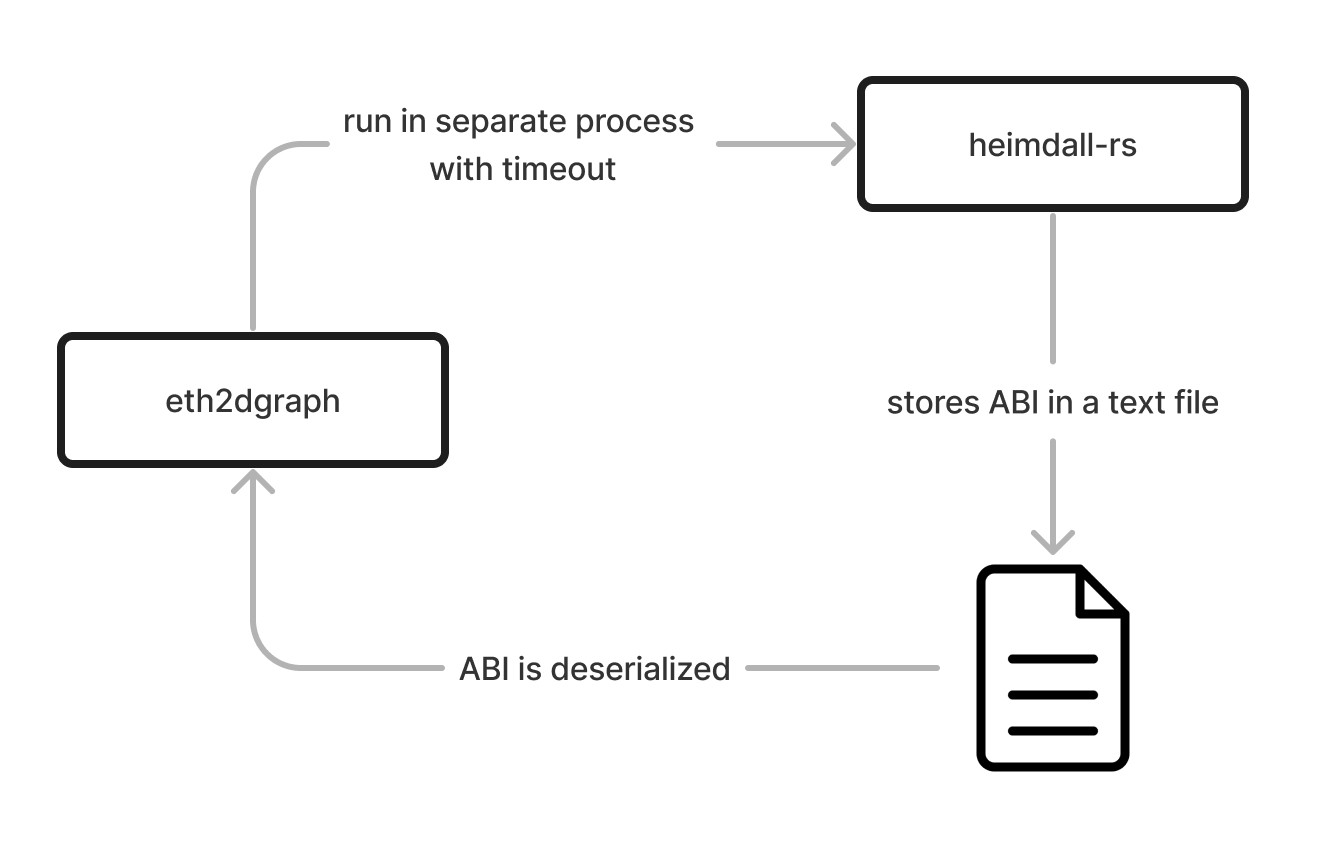
\includegraphics[width=1\textwidth]{Figures/methods/decompilation-architecture.jpg}
  \caption[Heimdall-rs integration into eth2dgraph]{Heimdall-rs integration into eth2dgraph}
  \label{fig:decompilation-architecture}
\end{figure}

It is possible to extract function names using a database of reverse hashes. Function selectors are stored in the bytecode as the first four bytes of the hash of the function's signature. It is possible to read these four bytes and see if there are matching signatures that were previously reverse-hashed. Heimdall-rs does this using the public etherface\footnote{Etherface is a database of Ethereum functions and event signatures, with related hashes, available at: \url{https://www.etherface.io/}} database. 
Unfortunately, it is not possible to extract parameter names from the bytecode stored on the blockchain. This piece of information is removed during the compilation of the code. 

Heimdall-rs is integrated in eth2graph using separate processes. Each time there is the need to run the decompiler, eth2dgraph creates a new process. This is done for isolation. For the nature of how the decompiler works, it can run in infinite loops during the symbolic execution. To avoid that, eth2dgraph has a parameter to set the maximum time spent waiting for de-compilation. The default is  five seconds.

The output of the {\tt heimdall-rs} process is stored in text files. When decompilation is done, these files are de-serialized by eth2dgraph into Rust data structures. \cref{fig:decompilation-architecture} shows how decompilation in handled in eth2dgraph.

\subsection{Contracts skeleton and metadata}
\label{skeleton-section}
The \textit{skeleton} of an EVM bytecode is the bytecode itself with all the arguments of the PUSH opcode set to zero. It allows to find bytecodes that are functionally identical between them. The concept of skeleton is used in many studies to reduce the total number of contracts to analyze~\cite{token-contracts}\cite{wallet-contracts}.

Removing the PUSH arguments to the bytecode deployed on the blockchain is not enough to extract the skeletons. The Solidity compiler can add metadata at the end of the bytecode that must be removed before getting the skeleton.  

Eth2dgraph identifies this part using a regular expression. Metadata is stored as CBOR\footnote{CBOR is a binary data serialization format standardized in RFC8949 \url{https://www.rfc-editor.org/rfc/rfc8949.html}} encoded data. After being split, the \textit{runtime} part of the bytecode is processed for the skeleton extraction, while the metadata part is decoded. Metadata are also stored in the indexed data, these are the field included:

\begin{itemize}
    \item \textit{storage\_protocol}: distributed file system protocol where the developer can eventually store the source code of the contract.
    \item \textit{storage\_hash}: location on the contract's data in the distributed file system.
    \item \textit{compiler}: the version of the Solidity compiler used.
    \item \textit{experimental}: whether the compilation was performed with experimental features activated.
\end{itemize}

The skeleton extraction is performed by looping through the bytes of the EVM bytecode. A byte between \texttt{0x60} and \texttt{0x7f} represents a PUSH instruction. If a byte is found in that range, the next bytes are replaced with zeros depending on the kind of PUSH found. 

\subsection{Verified source code}

It is possible to link contracts to their verified source code using the repository of \textit{Smart Contract Sanctuary}~\cite{smart_contract_sanctuary}. After cloning the repository locally, eth2dgraph can be run with an option to include the source code of the discovered contracts in the indexed data.

This allows querying the contracts based on text inside the source code. Dgraph supports text matching with stemming stop word removal. Data can be queried with two query functions: \texttt{anyoftext} and \texttt{alloftext}. The first function matches for any of the term searched for, while the second function matches for all the search terms.

A query example with {\tt anyoftext} is searching for all smart contracts that have in the source code the terms {\it token}, {\it erc20} or {\it erc721}. To be more precise, it would be possible to search with {\tt alloftext} all the smart contracts that have in the source code the exact signature of the transfer function of either the ERC20 or ERC721 standards. All of this is doable in a single fast query.

\subsection{Token transfers}

The ERC20 and ERC721 token standards state that when a token ownership is transferred an event MUST be emitted. \cref{lst:erc20-transfer} shows the event emitted for fungible token transfers, \cref{lst:erc721-transfer} shows the one emitted for NFT transfers. Emitting an event means generating a log that is indexed by Ethereum nodes.

\begin{lstlisting}[caption={Event emitted for ERC20 token transfer},label={lst:erc20-transfer},captionpos=b]
event Transfer(address indexed _from, address indexed _to, uint256 _value)
\end{lstlisting}

\begin{lstlisting}[caption={Event emitted for ERC721 token transfer},label={lst:erc721-transfer},captionpos=b]
event Transfer(address indexed _from, address indexed _to, uint256 indexed _tokenId)
\end{lstlisting}

Both events share the same name and type. The only difference is in the last parameter. It is indexed in the case of ERC721 and not indexed in the case of ERC20. The signature of the event is not influenced by this difference, so all the logs that describe token transfers share the same signature.

Logs with the first topic matching the {\tt keccak256} hash of the Transfer event signature are treated as token transfers by eth2dgraph.

After finding a matching log, the bytes composing the data field are split into 256-bit words and merged into the 256 words of the indexed topics.

The 256-bit words are then treated and decoded as follows:

\begin{itemize}
    \item First word is the \textit{from} address.
    \item Second word is the \textit{to} address.
    \item Third word is the \textit{value}. It represents the amount in the case of ERC20 or the token ID in the case of ERC721.
\end{itemize}

If the decoding succeeds, the log is parsed and later stored as a token transfer.

The distinction between ERC20 and ERC721 transfers is done based on the length of the topics array. Since ERC20 has the last parameter not indexed, the topic length is three words. For the ERC721 the topics length is four. This information is used to discriminate between storing the third word as \textit{value} or as \textit{token\_id}.

The same way of semantics extraction can be used for other kind of logs, e.g. token swaps. Eth2dgraph implements the code for parsing token transfer since it is the most common log emitted on the Ethereum chain.

\section{Software architecture}

The Ethereum network stores data in the order of billions of entries. The process of extraction must be as efficient as possible to be able to get this data in a reasonable time. At the time of writing, August 2023, Ethereum has 18M blocks. Performing every single action described in the previous sections sequentially for each block results in executions that take many days or even weeks. 

A lot of time is spent waiting for network data (the calls to the RPCs) or for the decompiler process to complete the decompilation. While it is not possible to make these steps faster, it is possible to parallelize them. Eth2dgraph has been developed to maximize concurrency of the machine where it is ran to minimize the time needed for data extraction.

This was done using async Rust and the \textit{Tokio asyncronous runtime}\footnote{Tokio provides a multi-threaded runtime for executing asynchronous Rust code \url{https://tokio.rs/}.}. \cref{fig:eth2dgraph-architecture} gives a general overview of how tasks are used and how they communicate.

\begin{figure}[H]
  \centering
  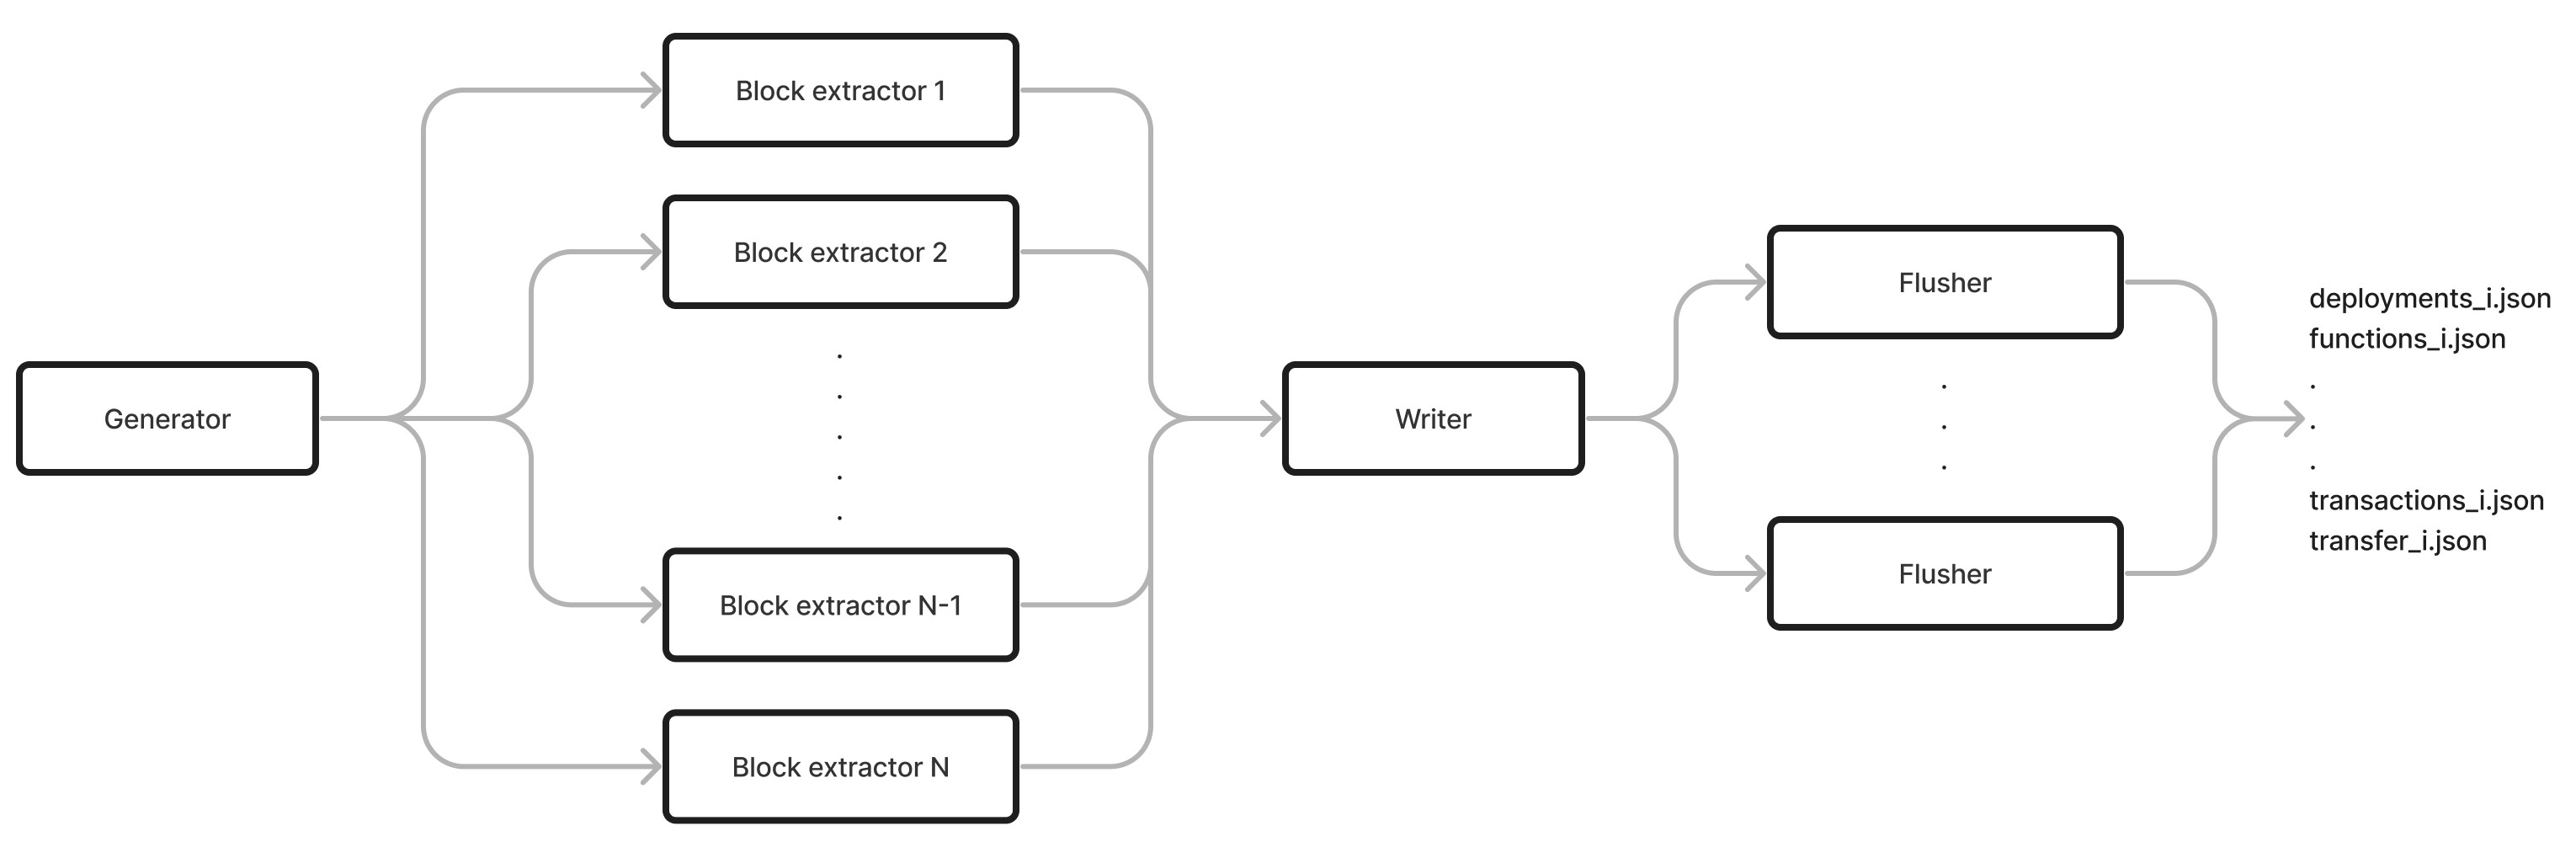
\includegraphics[width=1\textwidth]{Figures/methods/software-architecture.jpg}
  \caption[Software architecture of eth2dgraph]{Software architecture of eth2dgraph}
  \label{fig:eth2dgraph-architecture}
\end{figure}

Here is a more detailed description of each task:

\begin{itemize}
    \item The \textit{generator} task loops trough the block range to extract and spawns, using \texttt{tokio::spawn}, an \textit{extractor} task for each block that must be processed. It is also responsible for initializing all the data structures needed, the output data folders and the \textit{writer} task. 
    
    It is possible to set the limit of parallel extractor tasks to run usign the \texttt{--num-jobs} option. This is implemented using a semaphore. Each time an extractor task is created, it acquires a permit from a semaphore with a fixed capacity. When the task ends, the permit is dropped and, as a consequence, a new permit is freed in the semaphore. In case the maximum number of tasks is reached, the generator waits until the semaphore has a free permit available. This was done to avoid overloading the system with millions of concurrent tasks.

    \item The extractor task is the one responsible for the actual extraction. It receives as an argument the block to process and it collects all the data related to it. This includes handling the decompilation. All the steps related to data extraction were described in the previous sections.

    When data is ready to be stored, it is sent to the writer task using a bounded \textit{multiple-producer single-consumer} (mpsc) channel.

    \item The writer task is responsible to collect all the data sent by all the extractors and merge it. It stores data in buffers, one for each data type. When buffers reach a certain size, that can be set with the \texttt{--size-output} option, they are sent to a \textit{flusher} task to be stored to disk. The flusher tasks are spawned on demand by the writer task using \texttt{tokio::spawn\_blocking}. All their join handles are stored in a vector to wait for their termination at the end of the extraction.

    \item The flusher task is responsible for storing and compressing the output of the extraction. It receives a vector of a generic type \texttt{T} that implements the trait \texttt{SerializeDgraph}. It compresses this vector using gzip with a compression level that can be set as an option. Finally, it stores it in an output file. Data is stored divided by type and with incremental file names.
\end{itemize}

All these tasks are ran on the multi-threaded Tokio runtime. They are managed by the Tokio scheduler that implements a \textit{non-preemptive}, also called \textit{cooperative}, scheduling strategy. This means that tasks are switched when they explicitly ask for it, using \lstinline{.await}, giving back the control to the scheduler. 

In this way it is possible to maximize the parallelism of the extraction process. For example, when a task is downloading block's data, it calls \texttt{await} on the library function responsible for networking. This call tells the Tokio scheduler that the task is paused and cannot continue, so it is replaced with another task that has work to do. The task will be resumed when the network data is ready to be used.

\subsection{Decompilation cache}
\label{cachine-section}
One of the biggest bottlenecks of the extraction process was the decompilation step. Spawning a dedicated process for handling decompilation of all the 60M contracts takes a lot of time. The main problem is that the decompiler, for how it is designed, can encounter infinite loops during the building of the control flow graph. To avoid that, it is ran with a timeout of a few seconds, but even with that, it was slowing down the process by a lot.

The solution implemented in eth2dgraph is caching the decompilation based on bytecode skeletons. Two contract deployments sharing the same EVM skeleton are decompiled only once. The decompiled ABI of a skeleton comes from the decompilation of the first contract found with that skeleton.

The reason of this choice is that contracts sharing the same skeleton also share the same code logic. In theory, there could be a difference in the function names, since they are stored as arguments of PUSH instructions, but, from the data analyzed, this almost never happens.

To test the reliability of the caching logic, I compared ABIs extracted from decompiling each single contract to the ones got using the cache. To make the test more reliable, I ran it on various block ranges spanning trough the history of the Ethereum blockchain. \cref{table:caching-precision} reports the results of the tests. Full match means that the ABI got from the cache is exactly the same as the one got from a new decompilation run. Partial match indicates that the ABI got from the cache has the same exact function and event names, but there is at least one difference between types based on assumptions made by the decompiler (e.g. bytes instead of address). Mismatch indicates that the ABI got from the cache has at least one different function or event name.

\begin{table}[ht!]
\centering
    \begin{threeparttable}
    \begin{tabular}{m{3cm} m{2cm} m{2cm} m{2cm} m{2.5cm}} 
    \toprule
    \textbf{Blocks range} & \textbf{Cache hits} & \textbf{Full matches} & \textbf{Partial matches} & \textbf{Mismatches}   \\
    \midrule
    6000000-6001000   & 1373 & 1373 & 0 & 0 \\
    10000000-10001000 & 596 & 592 & 4 & 0 \\
    12008000-12009000 & 1296 & 1295 & 1 & 0 \\
    15505000-15506000 & 101 & 101 & 0 & 0 \\
    16001000-16002000 & 120 & 100 & 19 & 1 \\
    17000000-17001000 & 39 & 39 & 0 & 0 \\
    \bottomrule
    \end{tabular}
    \end{threeparttable}
    \caption{Precision of the decompilation caching logic}
    \label{table:caching-precision}
\end{table}

In total, 99.29\% of the cache hits resulted in full matches, 0.68\% in partial matches and just 0.03\% in mismatches.

This level of accuracy showed that caching decompilation based on skeletons is an effective way of reducing the time needed for semantics extraction. The slight loss of precision is justified by the boost in performance, that made it possible to scale the extraction of ABIs to all the history of the chain in a single machine. It allowed to reduce the number of decompilation runs from 60M to 470k.

The cache is implemented in the code with a shared \texttt{HashMap}. The implementation of the concurrent hashmap used is the one provided by the {\tt DashMap}\footnote{DashMap provides a concurrent hashmap that is faster and easier to use that the combination of {\tt RwLock} and {\tt HashMap}. It is available at:\url{https://github.com/xacrimon/dashmap}} crate. The \textit{key} of the hashmap is the hash of the skeleton's bytecode and the \textit{value} is an \textit{atomic unsigned integer}. The role of the number in the cache is of indicating how many failures that specific skeleton has encountered during decompilation. It is used for trying multiple times to decompile a skeleton that fails to decompile even with different contracts' bytecodes. These is an hard limit of ten attempts, after which the skeleton is stored without the ABI and no more decompilation processes will be spawned.

This way of extracting semantics has a direct implication on the schema of data. The ABI extracted by the decompiler is linked to the skeleton and not to the contract deployment itself. \cref{fig:contracts-storage} shows the result of this design choice in the schema.

\begin{figure}[H]
  \centering
  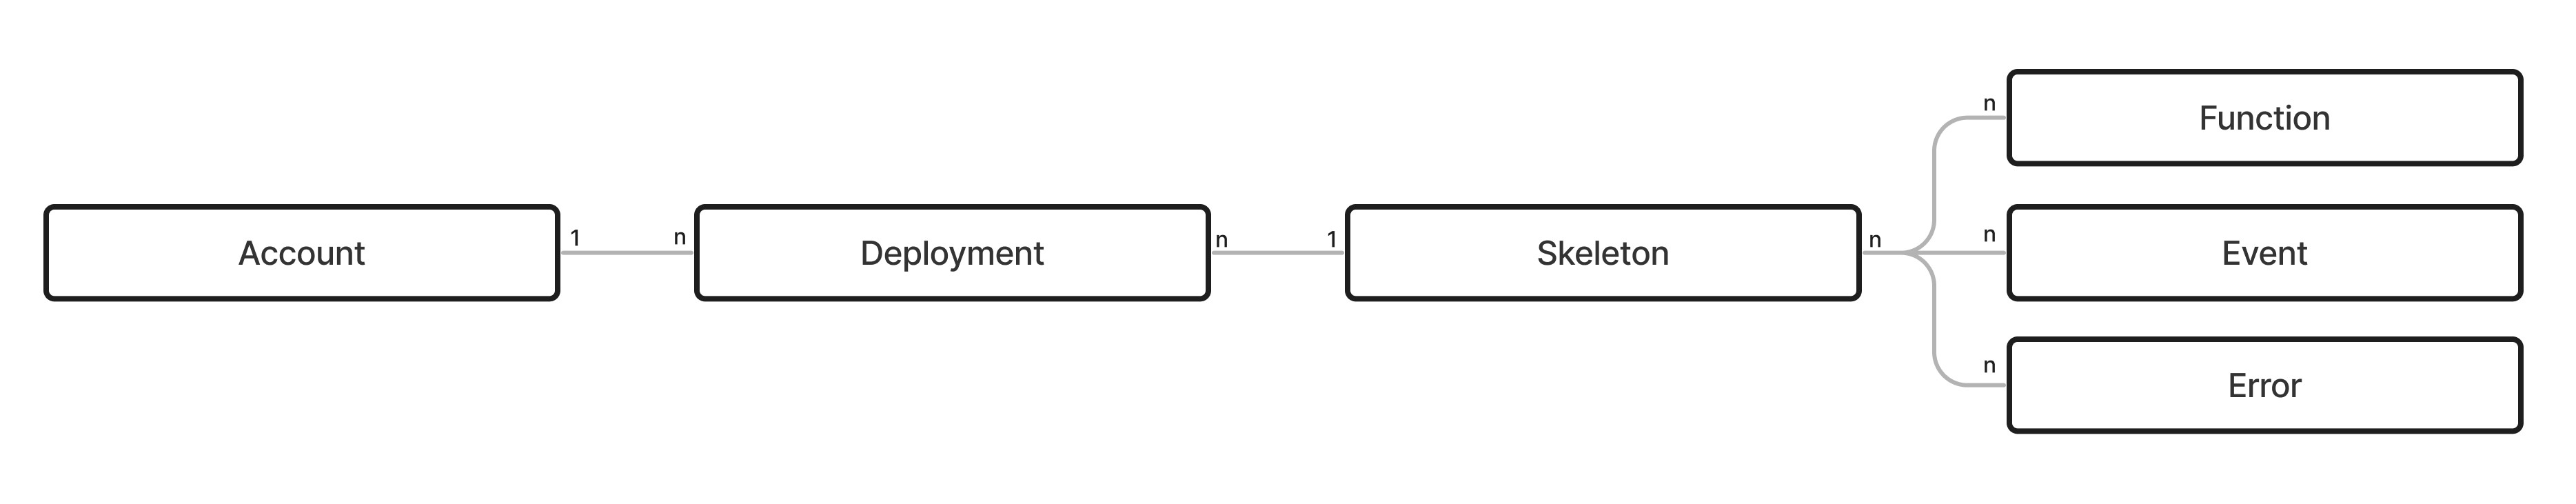
\includegraphics[width=1\textwidth]{Figures/methods/contracts-storage.jpg}
  \caption[Storage of contracts' information]{Storage of contracts' information}
  \label{fig:contracts-storage}
\end{figure}

\section{Similarity calculation}
\label{similarity-calculation}
Smart contracts' deployments are clustered based on bytecode skeletons: many smart contracts share the same skeleton and thus they are linked to the same skeleton entity in the database. To link these skeleton clusters together, some similarity metrics are needed. Linking skeleton clusters helps the process of data analysis; it ease the recognition of patterns and connections.

Eth2dgraph implements two similarity metrics:

\begin{itemize}
    \item \textit{Interface similarity}: inspired by Di Angelo and Salzer \cite{clustering-sc}, it calculates similarity between skeletons as the Jaccard index of the sets of function and event names. Two skeletons are similar if they have similar ABIs. It is calculated as 
    \begin{equation}
	Sim = \frac{|A\cap B|}{|A\cup B|}
    \end{equation}
    where $A$ and $B$ are the sets containing function and event names. It gives a number between $1$ (identical ABIs) and $0$ (non-overlapping ABIs).
    
    \item \textit{Bytecode similarity}: The interface similarity logic works greatly if the smart contracts implement many functions or events. It does not work very well if most of the code lies in internal functions and the exposed ones are just a few, like \texttt{start()} or \texttt{run()}. 
    To face this problem I added a second similarity metric that just considers the contracts' bytecodes. Inspired by Kiffer et al.~\cite{ethereum-sc-topology}, the metric used is the cosine similarity between hypervectors containing the frequencies of opcodes' 5-grams. It is computed as follows:
    \begin{enumerate}
        \item The two bytecodes to analyze are decoded to extract the opcodes, without their arguments.
        \item From the opcodes, the 5-grams and their frequencies are calculated. For example these instructions: 
        \begin{lstlisting}
PUSH1
PUSH1
MSTORE
CALLVALUE
DUP1
ISZERO
PUSH2
JUMPI
PUSH1\end{lstlisting}
        give these 5-grams with related frequencies as values:
        \begin{lstlisting}
[
    ("PUSH1 PUSH1 MSTORE CALLVALUE DUP1", 1),
    ("PUSH1 MSTORE CALLVALUE DUP1 ISZERO", 1),
    ("MSTORE CALLVALUE DUP1 ISZERO PUSH2", 1),
    ("CALLVALUE DUP1 ISZERO PUSH2 JUMPI", 1),
    ("DUP1 ISZERO PUSH2 JUMPI PUSH1", 1),
]       \end{lstlisting}
        \item This results in having two hypervectors, here called $A$ and $B$, in the dimension of the 5-grams. $A$ and $B$ are structured as shown in the previous listing. The cosine similarity is the cosine of the angle $\theta$ between these two vectors. It is possible to compute it as 
        \[
        cos(\theta)=\frac{A \cdot B}{||A||\,||B||}=\frac{\sum\limits_{i\in\Omega}A_iB_i}{ \sqrt{\sum\limits_{i\in\Omega}A^2_i \cdot \sum\limits_{i\in\Omega}B^2_i} }
        \]
        In the previous formula, $\Omega$ is the set that results from the intersection of the dimensions of $A$ and $B$.
        This gives a number between 0 (completely dissimilar bytecodes) and 1 (identical bytecodes). The suggested threshold for considering similarity suggested by Kiffer et al. is of $0.90$.
    \end{enumerate}
\end{itemize}

The process of similarity calculation is done on demand after data is loaded into Dgraph. The same binary that is responsible for the data extraction part also integrates commands to perform data analysis. 

It is possible to run eth2dgraph with the \texttt{analyse similarity} command to calculate both the previous metrics. Comparing all skeletons with each other is a heavy calculation, with a quadratic complexity with respect to the number of skeletons. It is possible to restrict the calculation to a single skeleton, giving as an argument the address of a contract.

To optimize the performances, calculation of similarity is done in parallel using the \textit{parallel iterators} of the \textit{Rayon}\footnote{Rayon is a data-parallelism library that easily introduces parallelism into existing sequential code  \url{https://docs.rs/rayon/latest/rayon/}} crate.

The output of the calculation is a text file containing the RDF triples that describe the similarities. It is possible to import it into the live database by running a mutation or using the Dgraph's \textit{live loader}.

Similarity values are stored as edge attributes, called \textit{facets} in Dgraph. It is possible to query the data filtering by similarity value. \cref{lst:skeleton-similarity-query} shows an example of how to retrieve similar skeletons filtering by similarity value.

\begin{lstlisting}[caption={Example DQL query for getting similar skeletons.},label={lst:skeleton-similarity-query},captionpos=b]
{
    q(func: uid(0x180c753f6)) {
        Skeleton.similar_code @facets(gt(similarity, 0.95)) @facets(similarity) {
            uid
        }
        Skeleton.similar_interface @facets(gt(similarity, 0.95)) @facets(similarity) {
            uid
        }
    }
}
\end{lstlisting}